\chapter{Transformer (2017)}

\begin{tcolorbox}
\fullcite{arxiv/1706.03762/Attention-Is-All-You-Need}
\end{tcolorbox}



\begin{enumerate}
    \item The (dominant) traditional sequence transduction models are based on complex recurrent or convolutional neural networks that include an encoder and a decoder.
    Some models also connect the encoder and decoder through an attention mechanism.
    \hfill \cite{arxiv/1706.03762/Attention-Is-All-You-Need}

    \item The Transformer, based solely on attention mechanisms, dispensing with recurrence and convolutions entirely. 
    \hfill \cite{arxiv/1706.03762/Attention-Is-All-You-Need}

    \item \textbf{Attention mechanisms} have become an integral part of compelling sequence modeling and transduction models in various tasks, allowing modeling of dependencies without regard to their distance in the input or output sequences.
    In all but a few cases, however, such attention mechanisms are used in conjunction with a recurrent network.
    \hfill \cite{arxiv/1706.03762/Attention-Is-All-You-Need}

    \item Transformer is a model architecture eschewing ($=$ avoiding) recurrence and instead relying entirely on an attention mechanism to draw global dependencies between input and output.
    \hfill \cite{arxiv/1706.03762/Attention-Is-All-You-Need}

    \item the number of operations required to relate signals from two arbitrary input or output positions (tokens) is a constant number of operations, albeit at the cost of reduced effective resolution due to averaging attention-weighted positions, an effect we counteract with Multi-Head Attention.
    \hfill \cite{arxiv/1706.03762/Attention-Is-All-You-Need}

    \item End-to-end memory networks are based on a recurrent attention mechanism instead of sequence-aligned recurrence and have been shown to perform well on simple-language question answering and language modeling tasks.
    \hfill \cite{arxiv/1706.03762/Attention-Is-All-You-Need}

\end{enumerate}





\section{Model Architecture (encoder-decoder)}

\begin{figure}[H]
    \centering
    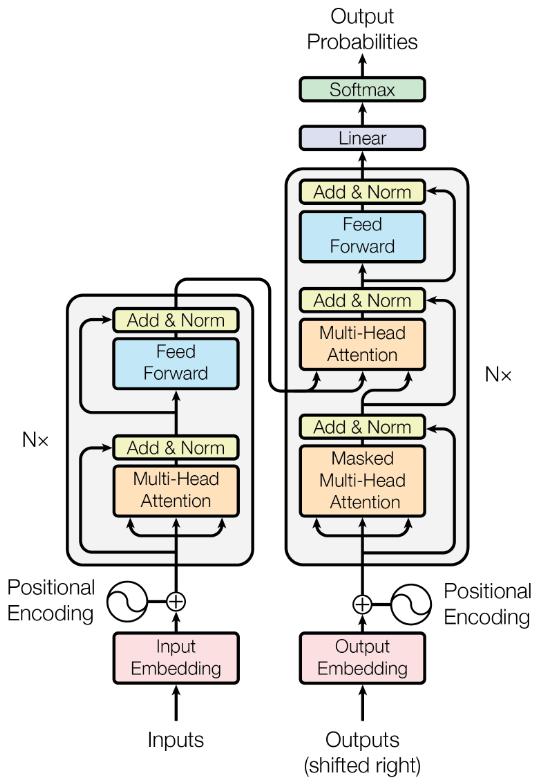
\includegraphics[
        width=\linewidth,
        height=10cm,
        keepaspectratio
    ]{images/advanced-ml/arxiv-1706.03762v7.fig-1.transformer-arch.png}
    \caption*{
        Transformer - model architecture \\
        left - encoder, right - decoder
        \cite{arxiv/1706.03762/Attention-Is-All-You-Need}
    }
\end{figure}


\begin{enumerate}
    \item the encoder maps an input sequence of symbol representations $(x_1, \cdots, x_n)$ to a sequence of continuous representations $\bm{z} = (z_1, \cdots, z_n)$. 
    Given $\bm{z}$, the decoder then generates an output sequence $(y_1, \cdots, y_m)$ of symbols one element at a time. 
    At each step the model is auto-regressive, consuming the previously generated symbols as additional input when generating the next.
    \hfill \cite{arxiv/1706.03762/Attention-Is-All-You-Need}

    \item The Transformer follows this overall architecture using stacked self-attention and point-wise, fully connected layers for both the encoder and decode.
    \hfill \cite{arxiv/1706.03762/Attention-Is-All-You-Need}

    % \item 
\end{enumerate}


\subsection{Encoder and Decoder Stacks}

\subsubsection*{Encoder}

\begin{enumerate}
    \item The encoder is composed of a stack of $N$ identical layers.
    \hfill \cite{arxiv/1706.03762/Attention-Is-All-You-Need}

    \item Each layer has two sub-layers. 
    The first is a \textbf{multi-head self-attention} mechanism, and 
    the second is a simple, position-wise fully connected feed-forward network.
    \hfill \cite{arxiv/1706.03762/Attention-Is-All-You-Need}

    \item We employ a residual connection around each of the two sub-layers, followed by layer normalization.
    That is, the output of each sub-layer is $\text{LayerNorm}(x + \text{Sublayer}(x))$, where $\text{Sublayer}(x)$ is the function implemented by the sub-layer itself. 
    \hfill \cite{arxiv/1706.03762/Attention-Is-All-You-Need}

    \item To facilitate these residual connections, all sub-layers in the model, as well as the embedding layers, produce outputs of dimension $d_{\text{model}}$.
    \hfill \cite{arxiv/1706.03762/Attention-Is-All-You-Need}
\end{enumerate}


\subsubsection*{Decoder}

\begin{enumerate}
    \item The decoder is composed of a stack of $N$ identical layers.
    \hfill \cite{arxiv/1706.03762/Attention-Is-All-You-Need}

    \item In addition to the two sub-layers in each encoder layer, the decoder inserts a third sub-layer, which performs \textbf{multi-head attention} over the output of the encoder stack.
    \hfill \cite{arxiv/1706.03762/Attention-Is-All-You-Need}

    \item we employ residual connections around each of the sub-layers, followed by layer normalization. 
    \hfill \cite{arxiv/1706.03762/Attention-Is-All-You-Need}

    \item We modify the self-attention sub-layer in the decoder stack to prevent positions from attending to subsequent positions.
    This masking, combined with fact that the output embeddings are offset by one position, ensures that the predictions for position $i$ can depend only on the known outputs at positions less than $i$.
    \hfill \cite{arxiv/1706.03762/Attention-Is-All-You-Need}
\end{enumerate}




\section{Applications of Attention in Transformer}

The Transformer uses multi-head attention in three different ways:

\begin{enumerate}
    \item In "encoder-decoder attention" layers, the queries come from the previous decoder layer, and the memory keys and values come from the output of the encoder. 
    This allows every position in the decoder to attend over all positions in the input sequence. 
    This mimics the typical encoder-decoder attention mechanisms in sequence-to-sequence models.
    \hfill \cite{arxiv/1706.03762/Attention-Is-All-You-Need}

    \item The encoder contains \textbf{self-attention layers}. 
    In a self-attention layer all of the keys, values and queries come from the same place, in this case, the output of the previous layer in the encoder. 
    Each position in the encoder can attend to all positions in the previous layer of the encoder.
    \hfill \cite{arxiv/1706.03762/Attention-Is-All-You-Need}

    \item Self-attention layers in the decoder allow each position in the decoder to attend to all positions in the decoder up to and including that position. 
    We need to prevent leftward information flow in the decoder to preserve the auto-regressive property. 
    We implement this inside of scaled dot-product attention by masking out (setting to $-\infty$) all values in the input of the softmax which correspond to illegal connections.
    \hfill \cite{arxiv/1706.03762/Attention-Is-All-You-Need}
\end{enumerate}




















